\documentclass[10pt,conference]{IEEEtran}
\usepackage[utf8]{inputenc}
\usepackage[english]{babel}
\usepackage{enumitem}
\usepackage{biblatex}
\usepackage[utf8]{inputenc}
\usepackage{graphicx}
\usepackage{multirow}
\usepackage{caption} 

\addbibresource{msr-challenge.bib}
\renewcommand\IEEEkeywordsname{Keywords}

\newlist{questions}{enumerate}{1}
\setlist[questions]{label*=\textbf{RQ\arabic*.}}

% correct bad hyphenation here
\hyphenation{op-tical net-works semi-conduc-tor}


\begin{document}

\title{Still need to find a title}


% author names and affiliations
% use a multiple column layout for up to three different
% affiliations
\author{\IEEEauthorblockN{Jasmine Latendresse}
\IEEEauthorblockA{Concordia University\\
Department of Computer Science and\\
Software Engineering\\
Montreal, Canada\\
Email: latendresse.jasmine@gmail.com}
\and
\IEEEauthorblockN{Rabe Abdalkareem}
\IEEEauthorblockA{Concordia University\\
Department of Computer Science and\\
Software Engineering\\
Montreal, Canada\\
Email: INCLUDE EMAIL}
\and
\IEEEauthorblockN{Diego Elias Costa}
\IEEEauthorblockA{Concordia University\\
Department of Computer Science and\\
Software Engineering\\
Montreal, Canada\\
Email: diego.costa@concordia.ca}}

% make the title area
\maketitle

% As a general rule, do not put math, special symbols or citations
% in the abstract
\begin{abstract}
Continuous Integration (CI) is the practice of automatically compiling, building, and testing code changes from multiple contributors to be integrated into a single code base. Program repair is one of the core processes in software development and becomes increasingly costly over time. Hence, the development community has adopted Continuous Integration (CI) as a way to push changes into production as quickly as possible by integrating often; allowing to detect and locate errors quickly. However, little is known about how effective Continuous Integration (CI) is at detecting simple, one-line bugs. Hence, in this paper, we analyze the coverage of Continuous Integration (CI), particularly, Travis CI---a popular CI service provider, for simple, one-line bugs and study the lifespan of such bugs in the code base. We find that 13 (out of 16) bug types are detected and that 16.12\% of bugs from open source projects are caught by the CI. We also find that simple, one-line bugs remain in the code base for a median time of 10.17 days before being fixed. This suggests that some bugs were immediately fixed and possibly never made it through the CI pipeline. More work is needed to determine why doesn't the CI catch certain bugs. 
\end{abstract}

\section{Introduction}
This is the introduction section. Here is a test citation \cite{abdalkareem_2020_a}. Some text to see the indentation of the research questions. Some more text to check the indentation of the research questions.
\begin{questions}
    \item How many bugs were caught by the CI? \\ We find that 16.1\% of the bugs are caught by the CI pipeline. Indeed, on a total of 273 distinct mapped bug---fix found in Commit Guru, 44 were either part of a push that triggered a build, or triggered a build. 
\end{questions}
\begin{questions}[resume]
    \item How long do bugs stay in the code? \\ On average, bugs stay in the code for 93.4 days with a median lifespan of 10.2 days. These results largely vary per bug type classification.  
\end{questions}

\section{Case Study Design}
\begin{figure*}[t]
\centering
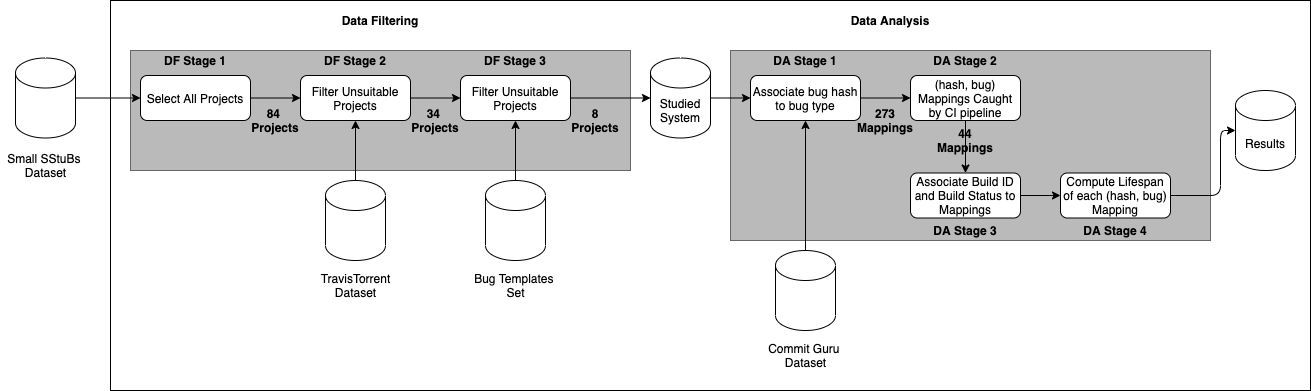
\includegraphics[width=\linewidth]{process.png}
\caption{An overview of our approach to study the MSR Challenge data set.}
\label{fig:process}
\end{figure*}

\subsection{Data Filtering}
How we selected the project for our analysis (how we filtered down to the 8 projects we have, what were the criteria, etc). Mention extraction of additional data from travis torrent and commit guru. Why we wanted travis torrent data (for CI data), why we needed commit guru data (to have additional data on the commit (bug) history.

\subsection{Data Analysis}

\section{Case Study Results}

\begin{table*}[t]
\centering
\begin{tabular}{lll}
\hline
Caught by Commit Guru         & Distinct (bug\_hash, fix\_hash, bug\_type) mappings     & 273    \\ \hline
\multirow{3}{*}{Caught by CI} & Build trigger, not in push commits                    & 8      \\
                              & In push commits, not a trigger                        & 17     \\
                              & Trigger or in push commits                            & 44     \\ \hline
Coverage                      & Distinct (bug\_hash, fix\_hash, bug\_type) caught by CI & 16.1\% \\ \hline
\end{tabular}
\caption{Distinct Bugs Caught by Travis CI.}
\label{tab:caughtbytravis}
\end{table*}

\begin{table*}[t]
\centering
\begin{tabular}{llll}
\hline
Caught by TravisTorrent            & Distinct (bug\_hash, fix\_hash, bug\_type, tr\_build\_id) mappings & 56 &        \\ \hline
\multirow{3}{*}{tr\_build\_status} & Pass                                                               & 34 & 60.7\% \\
                                   & Fail                                                               & 5  & 8.9\%  \\
                                   & Error                                                              & 17 & 30.4\% \\ \hline
\end{tabular}
\caption{Distinct Bugs---Builds Mappings Caught by Travis CI. }
\label{tab:buildstatus}
\end{table*}

%\begin{figure}[h]
%\includegraphics[width=\linewidth]{bugtypes.png}
%\caption{Proportion of Bug Types caught by the CI Pipeline.}
%\label{fig:process}
%\end{figure}

\begin{table*}[]
\centering
\begin{tabular}{lll}
\hline
Bug Type                           & Average Lifespan (days) & Median Lifespan (days) \\ \hline
CHANGE\_IDENTIFIER                 & 70,4                    & 10,2                   \\
OVERLOAD\_METHOD\_MORE\_ARGS       & 435,8                   & 435,8                  \\
CHANGE\_MODIFIER                   & 268,3                   & 8,46                   \\
DIFFERENT\_METHOD\_SAME\_ARGS      & 59,6                    & 7,4                    \\
CHANGE\_NUMERAL                    & 25,14                   & 6,4                    \\
CHANGE\_CALLER\_IN\_FUNCTION\_CALL & 13,2                    & 13,2                   \\
LESS\_SPECIFIC\_IF                 & 10,6                    & 10,6                   \\
OVERLOAD\_METHOD\_DELETED\_ARGS    & 68,6                    & 68,6                   \\
SWAP\_BOOLEAN\_LITERAL             & 67,9                    & 67,9                   \\
SWAP\_ARGUMENTS                    & 16,2                    & 16,2                   \\
CHANGE\_OPERAND                    & -                       & -                      \\
CHANGE\_UNARY\_OPERATOR            & -                       & -                      \\
DELETE\_THROWS\_EXCEPTION          & -                       & -                      \\
MORE\_SPECIFIC\_IF                 & -                       & -                      \\
ADD\_THROWS\_EXCEPTION             & -                       & -                      \\
CHANGE\_OPERATOR                   & -                       & -                      \\ \hline
\end{tabular}
\caption{Lifespan per Bug Type}
\label{tab:lifespan}
\end{table*}


\section{Conclusions}

\printbibliography

\end{document}


